%\documentclass[11pt,a4paper]{article}
\documentclass[11pt,a4paper]{scrartcl}
%\documentclass[11pt,a4paper,oneside]{book}
\usepackage[british,UKenglish,USenglish,english,american]{babel}
%\usepackage[a4paper, total={16cm, 23cm}]{geometry}
\usepackage[tmargin = 1.25in,bmargin = 1.25in,lmargin = 0.75in,rmargin = 0.75in]{geometry}
\usepackage{tikz}
\usepackage{graphicx}
\usepackage{pgfplots}
\pgfplotsset{width=12cm,compat=1.9}
\usepackage{setspace}
\usepackage{chemmacros}
\usepackage{chemfig}
%\usepackage{ghsystem}
\usechemmodule{redox}
%\usepackage{chemnum}
%\usepackage{bohr}
%\usepackage{elements}
%\usepackage{endiagram}
%\usepackage{modiagram}
%\usepackage{chemgreek}
%\usepackage{mhchem}
\usepackage{esint}
\usepackage{tabularray}

\usepackage{makeidx}
\usepackage{epstopdf}

\usepackage{amssymb}
\usepackage{mathrsfs}
%\usepackage{minted}
\usepackage{bm}
\usepackage{amsmath}
\usepackage{enumitem}
\usepackage[english]{varioref}
\usepackage[english]{babel}
\usepackage{lipsum}
\usepackage{fancyhdr}
\pagestyle{fancy} 
\usepackage{float}
\usepackage{empheq}
\usepackage[framemethod=tikz]{mdframed}
\usepackage{epstopdf}
\numberwithin{equation}{section}
\usepackage{eso-pic}
\usepackage{calc}
\usepackage{nccmath}
\usepackage{caption}
\usepackage{subcaption}
\usepackage{gensymb}
\usepackage{amsfonts,amsthm,epsfig,epstopdf,titling,url,array}
\usepackage{siunitx}
\sisetup{input-digits = 0123456789\pi}
\usepackage[symbol]{footmisc}
\usepackage{xcolor}
\usepackage{multicol}
\usepackage{boondox-cal}
\DeclareSIUnit\atm{atm}
\setcounter{secnumdepth}{3}
\setcounter{tocdepth}{3}
\usepackage{booktabs}
\usepackage{blindtext}
\usepackage{changepage}

% \usepackage{draftwatermark}
% \SetWatermarkText{DRAFT}
% \SetWatermarkScale{5}

\DeclareSIUnit\atm{atm}

\pagestyle{fancy} 
\fancypagestyle{firstpage}{
\rhead{
	\begin{picture}(0,0) 
			\put(-30,0){\includegraphics[width=1cm]{figures/logo_pemlab.eps}} 
	\end{picture}
}
}
\fancyhead[L]{\small\slshape\nouppercase{\leftmark}}
\chead{}
\rhead{
	\begin{picture}(0,0) 
		\put(-30,0){\includegraphics[width=1cm]{figures/logo_pemlab.eps}} 
	\end{picture}
}
\lfoot{\textit{}}
\cfoot{-\ \thepage\ -}
\rfoot{\textit{}}

\DeclareMathOperator{\rank}{rank}
\DeclareMathOperator{\atantwo}{atan2}
\DeclareMathOperator{\arctantwo}{arctan2}
\DeclareMathOperator{\spn}{span}

\renewcommand{\headrulewidth}{0.4pt}
\renewcommand{\footrulewidth}{0.4pt}
\newcommand{\abs}[1]{\left|#1\right|}
\definecolor{mycolor1}{rgb}{0.97, 0.97, 0.97}
\definecolor{mycolor2}{rgb}{0.97, 0.97, 0.97}
\definecolor{tableShade}{gray}{0.9}
\newcommand{\sign}{\text{sign}}
\newcommand{\centered}[1]{\begin{tabular}{@{}l@{}} #1 \end{tabular}}
\theoremstyle{it}
\newtheorem{defn}{Definition}[section]
\newtheorem{assumption}{Assumption}[section]
\newtheorem{thm}{Theorem}[section]
\newtheorem{lemma}{Lemma}[section]
\newtheorem{corollary}{Corollary}[section]
\theoremstyle{definition}
%\theoremstyle{it}
\newtheorem{example}{Example}[section]
\let\eqrefn\eqref
\renewcommand{\eqref}[1]{Eq.~(\ref{#1})}

\newenvironment{myitemize_1}
{ \begin{itemize}[topsep=4pt]
		\setlength{\topsep}{2pt}		
		\setlength{\itemsep}{2pt}
		\setlength{\parskip}{2pt}
		\setlength{\parsep}{2pt}     }
	{ \end{itemize}                  }


\newmdenv[innerlinewidth=0.5pt, roundcorner=4pt,backgroundcolor=mycolor2, 
linecolor=mycolor1,innerleftmargin=6pt,
innerrightmargin=6pt,innertopmargin=6pt,innerbottommargin=6pt]{mybox}

\title{\textbf{ 
	\begin{LARGE}
		Three Phase Inductors
	\end{LARGE} \\[24pt]
	\begin{Large}
		Mathematical Model and Construction
	\end{Large}}
}
\author{\textbf{Davide Bagnara}}

\begin{document}
	\thispagestyle{empty}
	\begin{mybox}
		\maketitle
		\vspace{150mm}
	\end{mybox}
%	\let\clearpage\relax
	\newpage
	\tableofcontents%
	\listoffigures%
	\listoftables
%	\let\clearpage\LaTeXStandardClearpage
	\newpage
	
\begin{onehalfspace}
	
	\pagebreak
	\section{Three phase inductance: mathematical model}
	\noindent\textbf{Three-phase inductance with four limbs}:
	\begin{figure}[H]
		\centering
		\includegraphics[width = 500pt, angle = 0, 
		keepaspectratio]{figures/three-phase-inductor-ver-i.eps}
		\captionsetup{width=0.75\textwidth, font=small}	
		\caption{Three-phase inductance: differential and common operational mode with four magnetic limbs.}
		\label{fig1}
	\end{figure}
	\noindent\textbf{Three-phase inductance with three limbs - pure differential mode}:
	\begin{figure}[H]
		\centering
		\includegraphics[width = 500pt, angle = 0, 
		keepaspectratio]{figures/three-phase-inductor-dm-ver-i.eps}
		\captionsetup{width=0.75\textwidth, font=small}	
		\caption{Three-phase inductance: pure differential operative mode with three magnetic limbs.}
		\label{fig2}
	\end{figure}
	
	\noindent\textbf{Three-phase inductance with one limb - pure common mode}:
	\begin{figure}[H]
		\centering
		\includegraphics[width = 500pt, angle = 0, 
		keepaspectratio]{figures/three-phase-inductor-cm-ver-i.eps}
		\captionsetup{width=0.75\textwidth, font=small}	
		\caption{Three-phase inductance: pure common operative mode with one magnetic limbs (classical toroidal core is used for low power application).}
		\label{fig3}
	\end{figure}
	\noindent\textbf{Mathematical model}:
	\begin{equation}\left\lbrace 
		\begin{aligned}
			u_u^{12}(t) &= u_u^{cm}(t)+u_u^{dm}(t) \\[6pt]
			u_v^{12}(t) &= u_v^{cm}(t)+u_v^{dm}(t) \\[6pt]
			u_w^{12}(t) &= u_w^{cm}(t)+u_w^{dm}(t) \\[6pt]
		\end{aligned}\right. 
	\end{equation}
	where
	\begin{equation}\left\lbrace 
		\begin{aligned}
			u_u^{dm}(t) + u_v^{dm}(t) + u_w^{dm}(t) &= 0 \\[6pt]
			\frac{1}{3}\Big(u_u^{cm}(t) + u_v^{cm}(t) + u_w^{cm}(t)\Big) &= u_{cm}(t) \\[6pt]
		\end{aligned}\right. 
	\end{equation}
	
	\begin{equation}\left\lbrace 
		\begin{aligned}
			u_u^{12}(t) -R i_u(t) - L_a \frac{d\,i_u}{dt}(t) + L_m \frac{d\,i_v}{dt}(t) + L_m \frac{d\,i_w}{dt}(t) &= 0 \\[6pt]
			u_v^{12}(t) -R i_v(t) - L_a \frac{d\,i_v}{dt}(t) + L_m \frac{d\,i_u}{dt}(t) + L_m \frac{d\,i_w}{dt}(t) &= 0 \\[6pt]
			u_w^{12}(t) -R i_w(t) - L_a \frac{d\,i_w}{dt}(t) + L_m \frac{d\,i_u}{dt}(t) + L_m \frac{d\,i_v}{dt}(t) &= 0 \\[6pt]
		\end{aligned}\right. 
	\end{equation}
	which results in matrix form
	\begin{equation}
		\vec{u}_{uvw}^{12}(t) - \mathbf{R}\vec{i}_{uvw}(t) - \mathbf{L}\frac{d}{dt}\vec{i}_{uvw}(t) = 0
	\end{equation}
	where
	\begin{equation}
		\mathbf{R} = \begin{bmatrix} R & 0 & 0 \\ 0 & R & 0 \\ 0 & 0 & R \end{bmatrix}, \qquad 
		\mathbf{L} = \begin{bmatrix} L_a & -L_m & -L_m \\ -L_m & L_a & -L_m \\ -L_m & -L_m & L_a \end{bmatrix}.
	\end{equation}
	in order to derive the equivalent \textit{differential} and \textit{common} mode equations the following transformation matrix is accounted
	\begin{equation}
		\mathbf{T} = \begin{bmatrix} 1 & -1 & 0 \\ 0 & 1 & -1 \\ -1 & 0 & 1 \\ \frac{1}{3} & \frac{1}{3} & \frac{1}{3} \end{bmatrix}.
	\end{equation}
	where
	\begin{equation}
		\vec{u}_{uvw}^{12} = \begin{bmatrix} u^{12}_{u}(t) \\[6pt] u^{12}_{v}(t) \\[6pt] u^{12}_{w}(t) \end{bmatrix}= \mathbf{T}^{-1}\begin{bmatrix} u^{dm}_{uv}(t) \\[6pt] u^{dm}_{vw}(t) \\[6pt] u^{dm}_{wu}(t) \\[6pt] u_{cm}(t) \end{bmatrix}.
	\end{equation}
	where
	\begin{equation}
		\begin{bmatrix} u^{dm}_{uv}(t) \\[6pt] u^{dm}_{vw}(t) \\[6pt] u^{dm}_{wu}(t) \\[6pt] u_{cm}(t) \end{bmatrix} - \begin{bmatrix} R & -R & 0 \\ 0 & R & -R \\ -R & 0 & R \\ R & R & R \end{bmatrix} \begin{bmatrix} i_u(t) \\ i_v(t) \\ i_w(t) \end{bmatrix} - \begin{bmatrix} L_a+L_m & -(L_a+L_m) & 0 \\ 0 & L_a+L_m & -(L_a+L_m) \\ -(L_a+L_m) & 0 & L_a+L_m \\ L_a-2L_m & L_a-2L_m & L_a-2L_m \end{bmatrix} \begin{bmatrix} \frac{di_u}{dt}(t) \\ \frac{di_v}{dt}(t) \\ \frac{di_w}{dt}(t) \end{bmatrix} = 0
	\end{equation}
	expressing in terms of $\begin{bmatrix} u^{12}_{dmu}(t) & u^{12}_{dmv}(t) & u^{12}_{dmu}(t) \end{bmatrix}^{T}$ and $u_{cm}(t)$ we obtain the following system
	
	\begin{equation}
		\vec{u}_{duvw}^{12}(t) - \mathbf{R}\vec{i}_{uvw}(t) - \mathbf{L}_{dm}\frac{d}{dt}\vec{i}_{uvw}(t) = 0
	\end{equation}
	where
	\begin{equation}
		\mathbf{R} = \begin{bmatrix} R & 0 & 0 \\ 0 & R & 0 \\ 0 & 0 & R \end{bmatrix}, \qquad 
		\mathbf{L} = \begin{bmatrix} L_a+L_m & 0 & 0 \\ 0 & L_a+L_m & 0 \\ 0 & 0 & L_a+L_m \end{bmatrix}.
	\end{equation}
	and 
	\begin{equation}
		{u}_{cm}(t) - R {i}_{cm}(t) - (L_a-2L_m)\frac{d}{dt}{i}_{cm}(t) = 0
	\end{equation}
	where ${i}_{cm}(t) = \frac{1}{3}\Big(i_u(t)+i_v(t)+i_w(t)\Big)$.
	Hence, in a three-phase inductance we have two inductive contributions
	\begin{itemize}
		\item[--] differential mode (also called \textit{positive sequence inductance}) given by $L_p = L_a + L_m$;
		\item[--] common mode (also called \textit{zero sequence inductance}) given by $L_0 = L_a -2L_m$
	\end{itemize}
	where $L_a$ is the self-inductance, and $L_m$ is the mutual-inductance.
	
	The relation between sequence values and machine values can be summarized as follows
	\begin{equation}\left\lbrace 
		\begin{aligned}
			L_p &= L_a + L_m \\[6pt]
			L_0 &= L_a -2L_m  \\[6pt]
			L_m &= \frac{1}{3}\Big(L_p - L_0\Big) \\[6pt]
			L_a &= \frac{1}{2}\Big(L_p + L_0 + L_m\Big) \\[6pt]
		\end{aligned}\right. 
	\end{equation}
	
	Commercially speaking three-phase inductor can be either \textit{common mode} or \textit{differential mode}:
	\begin{itemize}
		\item[--] Typically three-phase three-limbs inductors present only differential inductance. The residual common mode inductance is associated to the leakage inductance, see Figure~\ref{fig2}.
		\item[--] Typically three-phase common mode inductors are built around a common single limb core. The residual differential mode inductance is associated to the leakage inductance, see Figure~\ref{fig3}.
	\end{itemize}
	
	\section{Saturation effects}
	The saturation effects can be modelized assuming $L_a$ and $L_m$ as function of the current, as follows
	\begin{equation}\left\lbrace 
		\begin{aligned}
			L_{au} &= L_a^{nom} k_{sat}^{a}(i_u) + L_{a0}\rightarrow L_{a0}\quad\text{for } i\gg i_{sat}  \\[6pt]
			L_{av} &= L_a^{nom} k_{sat}^{a}(i_v) + L_{a0}\rightarrow L_{a0}\quad\text{for } i\gg i_{sat}  \\[6pt]
			L_{aw} &= L_a^{nom} k_{sat}^{a}(i_w) + L_{a0}\rightarrow L_{a0}\quad\text{for } i\gg i_{sat}  \\[6pt]
			L_{mu} &= L_m^{nom} k_{sat}^{m}(i_u) + L_{m0}\rightarrow L_{m0}\quad\text{for } i\gg i_{sat}  \\[6pt]
			L_{mv} &= L_m^{nom} k_{sat}^{m}(i_v) + L_{m0}\rightarrow L_{m0}\quad\text{for } i\gg i_{sat}  \\[6pt]
			L_{mw} &= L_m^{nom} k_{sat}^{m}(i_w) + L_{m0}\rightarrow L_{m0}\quad\text{for } i\gg i_{sat}  \\[6pt]
		\end{aligned}\right. 
	\end{equation}
	where $L_{a0}$ and $L_{m0}$ are the equivalent self and mutual inductance in air, condition which raises e.g. during short circuit current. 
	\begin{figure}[H]
		\centering
		\includegraphics[width = 300pt, angle = 0, 
		keepaspectratio]{figures/saturation-curve-ver-i.eps}
		\captionsetup{width=0.75\textwidth, font=small}	
		\caption{Saturation curve applied to $L_a$ and $L_m$, self and mutual inductance respectively.}
		\label{fig4}
	\end{figure}
	
	
	\begin{equation}
		\mathbf{L}(\vec{i}_{uvw}) = \begin{bmatrix} L_{ls}+L_a^{nom} k_{sat}^{a}(i_u) + L_{a0} & -\big[L_m^{nom} k_{sat}^{m}(i_v) + L_{m0}\big] & -\big[L_m^{nom} k_{sat}^{m}(i_w) + L_{m0}\big] \\[6pt] -\big[L_m^{nom} k_{sat}^{m}(i_u) + L_{m0}\big] & L_{ls}+L_a^{nom} k_{sat}^{a}(i_v) + L_{a0} & -\big[L_m^{nom} k_{sat}^{m}(i_w) + L_{m0}\big] \\[6pt] -\big[L_m^{nom} k_{sat}^{m}(i_u) + L_{m0}\big] & -\big[L_m^{nom} k_{sat}^{m}(i_v) + L_{m0}\big] & L_{ls}+L_a^{nom} k_{sat}^{a}(i_w) + L_{a0} \end{bmatrix}
	\end{equation}
	
	\newpage
	\begin{thebibliography}{9}
		\bibitem{heldwein} 
		M. L. Heldwein, L. Dalessandro, J. W. Kolar - \emph{The Three-Phase Common-Mode Inductor: Modeling Design Issues}. IEEE Transactions on industrial electronics, vol. 58, no. 8, August 2011.
		\bibitem{Hurley} 
		W. G. Hurley, W. H. Woelfle - \emph{Transformers and Inductors for Power Electronics. Theory design and applications}. J. Wiley 2013.
	\end{thebibliography}
	
	%*********************************************************
	% Print bibliography (If bibliography is empty nothing happens)
	%*********************************************************
	%\newpage
	%\printbibliography[heading=bibintoc]
\end{onehalfspace}
\end{document} 